\documentclass[10pt]{article}
\usepackage[utf8]{inputenc}
\usepackage[margin=0in,paperwidth=12in,paperheight=4in]{geometry}
\usepackage{tikz}
\usepackage{xcolor}
\usepackage{amsmath,amssymb}
\usetikzlibrary{shapes.geometric, arrows.meta, positioning, calc, backgrounds}
\pagestyle{empty}

\definecolor{bgdark}{HTML}{0F172A}
\definecolor{cardbg}{HTML}{1E293B}
\definecolor{bordercol}{HTML}{334155}
\definecolor{accentblue}{HTML}{38BDF8}
\definecolor{accentgreen}{HTML}{10B981}
\definecolor{accentorange}{HTML}{F59E0B}
\definecolor{accentpurple}{HTML}{A855F7}
\definecolor{accentred}{HTML}{EF4444}
\definecolor{accentcyan}{HTML}{06B6D4}
\definecolor{textwhite}{HTML}{F8FAFC}
\definecolor{textmuted}{HTML}{94A3B8}

\begin{document}
\noindent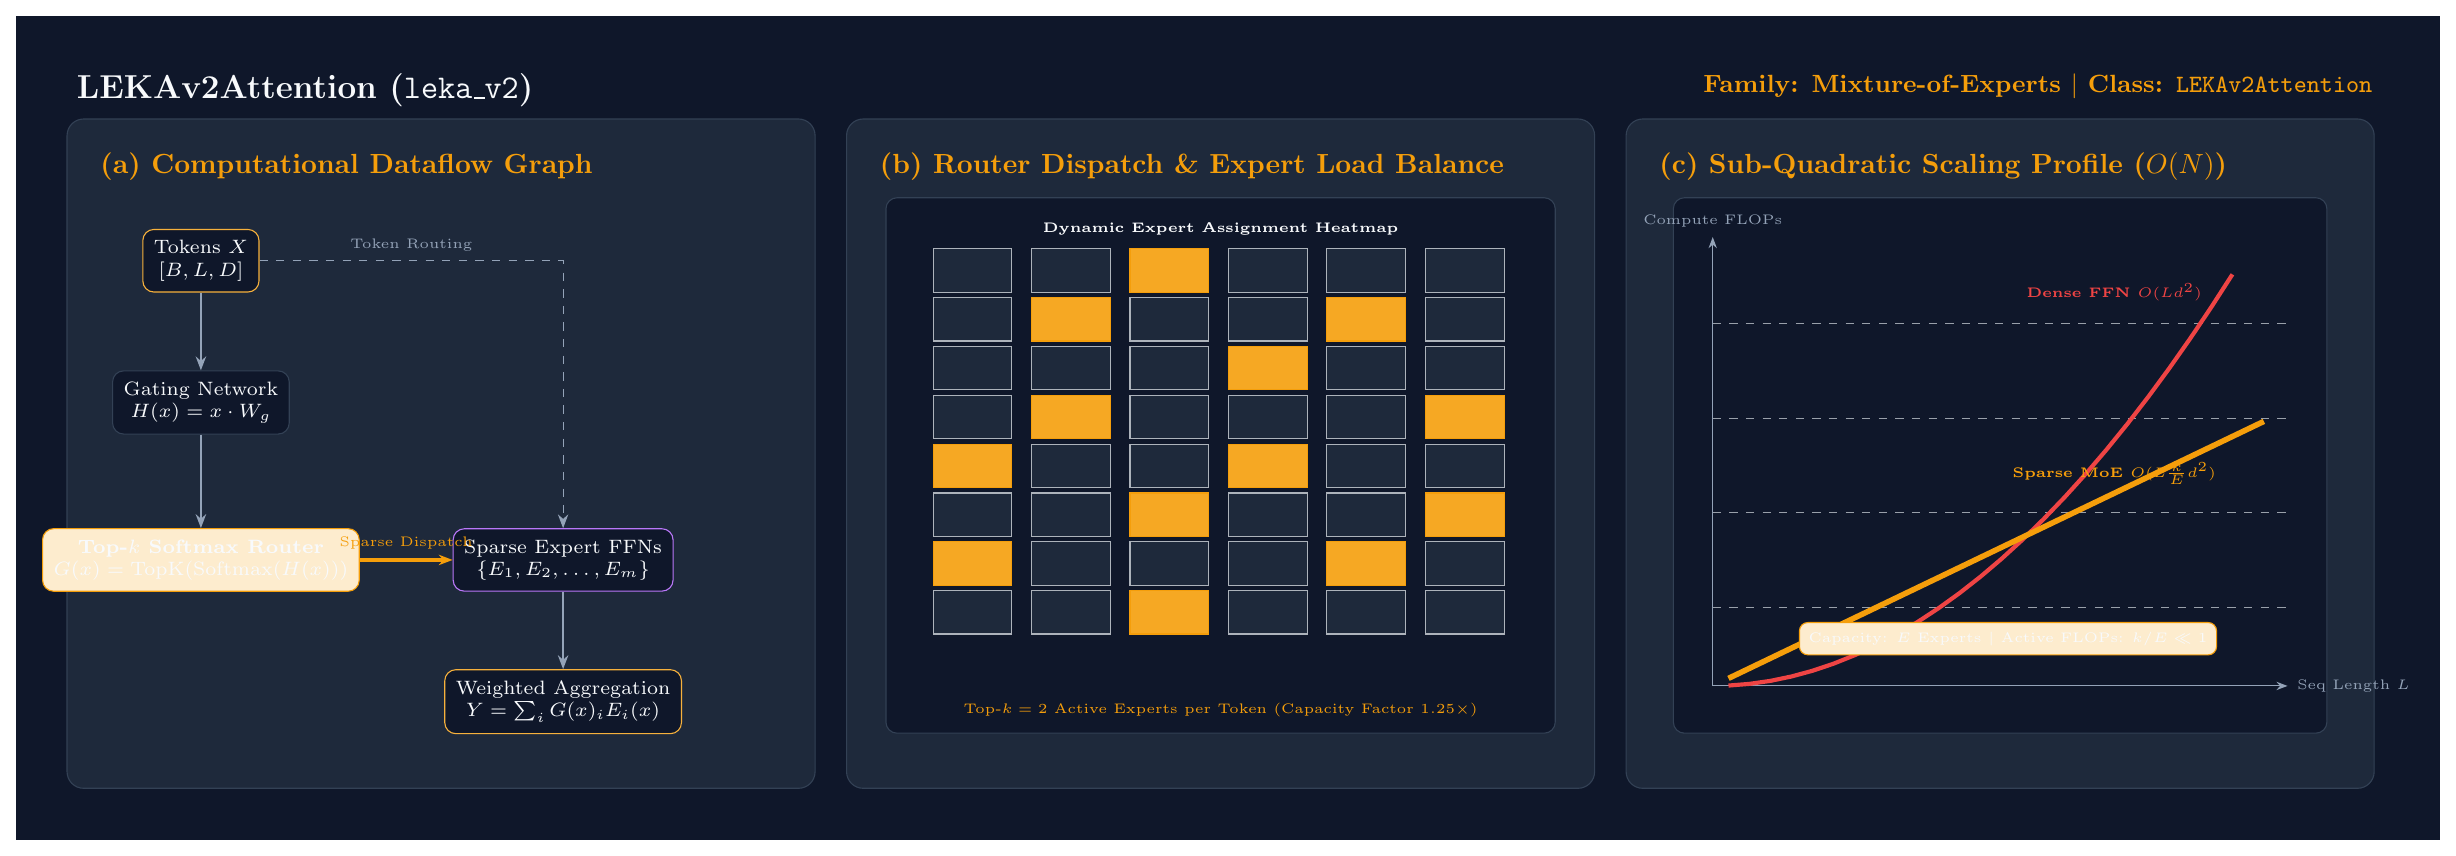
\begin{tikzpicture}[
    background rectangle/.style={fill=bgdark}, show background rectangle,
    scale=1.0, every node/.style={transform shape}
]

\clip (0,0) rectangle (30.48, 10.16);

% Title Header
\node[anchor=north west, text=textwhite, font=\large\bfseries] at (0.5, 9.7) {LEKAv2Attention (\texttt{leka\_v2})};
\node[anchor=north east, text=accentorange, font=\small\bfseries] at (29.9, 9.7) {Family: Mixture-of-Experts $\mid$ Class: \texttt{LEKAv2Attention}};

% Panel A: Computational Architecture
\draw[fill=cardbg, draw=bordercol, rounded corners=6pt] (0.5, 0.5) rectangle (10.0, 9.0);
\node[anchor=north west, text=accentorange, font=\bfseries\normalsize] at (0.8, 8.7) {(a) Computational Dataflow Graph};

\node[draw=accentorange!80, fill=bgdark, rounded corners=4pt, text=textwhite, font=\scriptsize, align=center, inner sep=4pt] (inp) at (2.2, 7.2) {Tokens $X$\\$[B, L, D]$};
\node[draw=bordercol, fill=bgdark, rounded corners=4pt, text=textwhite, font=\scriptsize, align=center, inner sep=4pt] (proj) at (2.2, 5.4) {Gating Network\\$H(x) = x \cdot W_g$};
\node[draw=accentorange, fill=accentorange!20, rounded corners=4pt, text=textwhite, font=\scriptsize\bfseries, align=center, inner sep=4pt] (core) at (2.2, 3.4) {Top-$k$ Softmax Router\\$G(x) = \mathrm{TopK}(\mathrm{Softmax}(H(x)))$};
\node[draw=accentpurple!80, fill=bgdark, rounded corners=4pt, text=textwhite, font=\scriptsize, align=center, inner sep=4pt] (gate) at (6.8, 3.4) {Sparse Expert FFNs\\$\{E_1, E_2, \dots, E_m\}$};
\node[draw=accentorange!80, fill=bgdark, rounded corners=4pt, text=textwhite, font=\scriptsize, align=center, inner sep=4pt] (outp) at (6.8, 1.6) {Weighted Aggregation\\$Y = \sum_i G(x)_i E_i(x)$};

        \draw[-{Stealth[length=5pt]}, textmuted, line width=1pt] (inp) -- (proj);
        \draw[-{Stealth[length=5pt]}, textmuted, line width=1pt] (proj) -- (core);
        \draw[-{Stealth[length=5pt]}, accentorange, line width=1.2pt] (core) -- (gate) node[midway, above, text=accentorange, font=\tiny] {Sparse Dispatch};
        \draw[-{Stealth[length=5pt]}, textmuted, line width=1pt] (gate) -- (outp);
        \draw[-{Stealth[length=5pt]}, dashed, textmuted] (inp) -| (gate) node[pos=0.25, above, font=\tiny] {Token Routing};
        

% Panel B: Structural Pattern & Dynamics
\draw[fill=cardbg, draw=bordercol, rounded corners=6pt] (10.4, 0.5) rectangle (19.9, 9.0);
\node[anchor=north west, text=accentorange, font=\bfseries\normalsize] at (10.7, 8.7) {(b) Router Dispatch \& Expert Load Balance};
\draw[draw=bordercol, fill=bgdark, rounded corners=4pt] (10.9, 1.2) rectangle (19.4, 8.0);
\node[text=textwhite, font=\tiny\bfseries] at (15.15, 7.6) {Dynamic Expert Assignment Heatmap};
\draw[fill=cardbg, draw=bordercol!40] (11.50, 6.80) rectangle (12.50, 7.35);
\draw[fill=cardbg, draw=bordercol!40] (12.75, 6.80) rectangle (13.75, 7.35);
\draw[fill=accentorange!90, draw=accentorange] (14.00, 6.80) rectangle (15.00, 7.35);
\draw[fill=cardbg, draw=bordercol!40] (15.25, 6.80) rectangle (16.25, 7.35);
\draw[fill=cardbg, draw=bordercol!40] (16.50, 6.80) rectangle (17.50, 7.35);
\draw[fill=cardbg, draw=bordercol!40] (17.75, 6.80) rectangle (18.75, 7.35);
\draw[fill=cardbg, draw=bordercol!40] (11.50, 6.18) rectangle (12.50, 6.73);
\draw[fill=accentorange!90, draw=accentorange] (12.75, 6.18) rectangle (13.75, 6.73);
\draw[fill=cardbg, draw=bordercol!40] (14.00, 6.18) rectangle (15.00, 6.73);
\draw[fill=cardbg, draw=bordercol!40] (15.25, 6.18) rectangle (16.25, 6.73);
\draw[fill=accentorange!90, draw=accentorange] (16.50, 6.18) rectangle (17.50, 6.73);
\draw[fill=cardbg, draw=bordercol!40] (17.75, 6.18) rectangle (18.75, 6.73);
\draw[fill=cardbg, draw=bordercol!40] (11.50, 5.56) rectangle (12.50, 6.11);
\draw[fill=cardbg, draw=bordercol!40] (12.75, 5.56) rectangle (13.75, 6.11);
\draw[fill=cardbg, draw=bordercol!40] (14.00, 5.56) rectangle (15.00, 6.11);
\draw[fill=accentorange!90, draw=accentorange] (15.25, 5.56) rectangle (16.25, 6.11);
\draw[fill=cardbg, draw=bordercol!40] (16.50, 5.56) rectangle (17.50, 6.11);
\draw[fill=cardbg, draw=bordercol!40] (17.75, 5.56) rectangle (18.75, 6.11);
\draw[fill=cardbg, draw=bordercol!40] (11.50, 4.94) rectangle (12.50, 5.49);
\draw[fill=accentorange!90, draw=accentorange] (12.75, 4.94) rectangle (13.75, 5.49);
\draw[fill=cardbg, draw=bordercol!40] (14.00, 4.94) rectangle (15.00, 5.49);
\draw[fill=cardbg, draw=bordercol!40] (15.25, 4.94) rectangle (16.25, 5.49);
\draw[fill=cardbg, draw=bordercol!40] (16.50, 4.94) rectangle (17.50, 5.49);
\draw[fill=accentorange!90, draw=accentorange] (17.75, 4.94) rectangle (18.75, 5.49);
\draw[fill=accentorange!90, draw=accentorange] (11.50, 4.32) rectangle (12.50, 4.87);
\draw[fill=cardbg, draw=bordercol!40] (12.75, 4.32) rectangle (13.75, 4.87);
\draw[fill=cardbg, draw=bordercol!40] (14.00, 4.32) rectangle (15.00, 4.87);
\draw[fill=accentorange!90, draw=accentorange] (15.25, 4.32) rectangle (16.25, 4.87);
\draw[fill=cardbg, draw=bordercol!40] (16.50, 4.32) rectangle (17.50, 4.87);
\draw[fill=cardbg, draw=bordercol!40] (17.75, 4.32) rectangle (18.75, 4.87);
\draw[fill=cardbg, draw=bordercol!40] (11.50, 3.70) rectangle (12.50, 4.25);
\draw[fill=cardbg, draw=bordercol!40] (12.75, 3.70) rectangle (13.75, 4.25);
\draw[fill=accentorange!90, draw=accentorange] (14.00, 3.70) rectangle (15.00, 4.25);
\draw[fill=cardbg, draw=bordercol!40] (15.25, 3.70) rectangle (16.25, 4.25);
\draw[fill=cardbg, draw=bordercol!40] (16.50, 3.70) rectangle (17.50, 4.25);
\draw[fill=accentorange!90, draw=accentorange] (17.75, 3.70) rectangle (18.75, 4.25);
\draw[fill=accentorange!90, draw=accentorange] (11.50, 3.08) rectangle (12.50, 3.63);
\draw[fill=cardbg, draw=bordercol!40] (12.75, 3.08) rectangle (13.75, 3.63);
\draw[fill=cardbg, draw=bordercol!40] (14.00, 3.08) rectangle (15.00, 3.63);
\draw[fill=cardbg, draw=bordercol!40] (15.25, 3.08) rectangle (16.25, 3.63);
\draw[fill=accentorange!90, draw=accentorange] (16.50, 3.08) rectangle (17.50, 3.63);
\draw[fill=cardbg, draw=bordercol!40] (17.75, 3.08) rectangle (18.75, 3.63);
\draw[fill=cardbg, draw=bordercol!40] (11.50, 2.46) rectangle (12.50, 3.01);
\draw[fill=cardbg, draw=bordercol!40] (12.75, 2.46) rectangle (13.75, 3.01);
\draw[fill=accentorange!90, draw=accentorange] (14.00, 2.46) rectangle (15.00, 3.01);
\draw[fill=cardbg, draw=bordercol!40] (15.25, 2.46) rectangle (16.25, 3.01);
\draw[fill=cardbg, draw=bordercol!40] (16.50, 2.46) rectangle (17.50, 3.01);
\draw[fill=cardbg, draw=bordercol!40] (17.75, 2.46) rectangle (18.75, 3.01);
\node[text=accentorange, font=\tiny] at (15.15, 1.5) {Top-$k=2$ Active Experts per Token (Capacity Factor $1.25\times$)};

% Panel C: Complexity / Scaling Profile
\draw[fill=cardbg, draw=bordercol, rounded corners=6pt] (20.3, 0.5) rectangle (29.8, 9.0);
\node[anchor=north west, text=accentorange, font=\bfseries\normalsize] at (20.6, 8.7) {(c) Sub-Quadratic Scaling Profile ($O(N)$)};

\draw[draw=bordercol, fill=bgdark, rounded corners=4pt] (20.9, 1.2) rectangle (29.2, 8.0);
\draw[-{Stealth[length=4pt]}, textmuted] (21.4, 1.8) -- (28.7, 1.8) node[right, font=\tiny, text=textmuted] {Seq Length $L$};
\draw[-{Stealth[length=4pt]}, textmuted] (21.4, 1.8) -- (21.4, 7.5) node[above, font=\tiny, text=textmuted] {Compute FLOPs};

\foreach \y in {2.8, 4.0, 5.2, 6.4} {
    \draw[dashed, bordercol!50] (21.4, \y) -- (28.7, \y);
}

        \draw[color=accentred, line width=1.5pt, domain=21.6:28.0] plot (\x, {1.8 + 0.12*(\x-21.4)*(\x-21.4)});
        \node[text=accentred, font=\tiny\bfseries] at (26.5, 6.8) {Dense FFN $O(L d^2)$};
        \draw[color=accentorange, line width=2pt, domain=21.6:28.4] plot (\x, {1.8 + 0.48*(\x-21.4)});
        \node[text=accentorange, font=\tiny\bfseries] at (26.5, 4.5) {Sparse MoE $O(L \frac{k}{E} d^2)$};
        \node[draw=accentorange, fill=accentorange!20, rounded corners=3pt, text=textwhite, font=\tiny] at (25.15, 2.4) {Capacity: $E$ Experts $\mid$ Active FLOPs: $k/E \ll 1$};
        

\end{tikzpicture}
\end{document}
